\chapter{Inputs}
\label{chap:1}

In this chapter, the input requirements, such as their format, are discussed. Also the input data table is described. Before running the code, the next chapter, Chapter \ref{chap:3}, should be read.

\section{Input data table}
To be able to use this tool, an input data table needs to be created first. This can be done manually in MySQL, but is recommended to do with the help of script called Create\_Dummy\_Database.py with the input file (Login\_Data.txt). It creates a table with 15 columns and 3 rows of dummy data with a  table name INPUT\_Table. The dummy data can be changed inside the python scrip, or just deleted after the table is made by calling the command in the command prompt:\\ TRUNCATE TABLE table name;\\

New input data can be added into the input table by running the Import\_New\_Data\_To\_Input\_Table \_MySQL.py script with Login\_Data.txt and Add\_Data.txt as inputs. This can be done in Python by calling: \\ Import\_New\_Data\_To\_Input\_Table\_MySQL.Import\_new\_data\_into\_input\_table('Login\_Data.txt','Add\_da-ta.txt')\\
after importing Import\_New\_Data\_To\_Input\_Table\_MySQL or from the command line by calling the file name. This adds data into a table called INPUT\_Table. Therefore, if the user changed the name of the input table it will create an error. \\

The format of the table is 15 columns, as seen in Figure \ref{fig:1}: OBS\_id, Observation\_date, Instrument, Mode, Vertex1\_1, Vertex1\_2, Vertex2\_1, Vertex2\_2, Vertex3\_1, Vertex3\_2, Vertex4\_1, Vertex4\_2, Status, Number\_of\_Asteroids \_Detected, Time\_Updated\_UTC\\
The OBS\_id is a specific id made up of the field of view, date and instrument, but can be also chosen at random. This is the primary key of the table. \\

\begin{figure}[h]
    \centering
    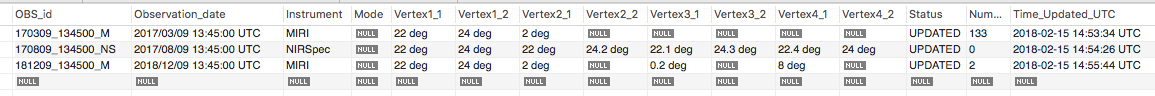
\includegraphics[width=1\textwidth]{Figures/Inputtable.png}
    \caption{The dummy Input table}
    \label{fig:1}
\end{figure}

Observation\_date is the date and time as which the sky is observed. This is given in the format as shown in Figure \ref{fig:1} with the time zone specified. Instrument and mode are information about which instrument at which mode was used.\\

The Vertex 1-4 are the four vertices of the field of view. Vertex1\_1 and Vertex1\_2 specify the RA and DEC for Vertex1. It is possible to use 3 different shapes for the field of view, polygon, circle and rectangle. Polygon consists of 4 vertices, each of RA and DEC. Circle has a field of view center (RA,DEC) and an angle specifying the radius. Rectangle had a field of view center (RA,DEC) and 3 angles. The values should be given with units as well, as can be seen in Figure \ref{fig:1}\\

Status is NULL at first, but after the tool is used, it is updated to UPDATED and the asteroids found in the field of view are counted and given in the next column.\\

The Time\_Updated\_UTC gives the date and time when the row was updated in UTC. This is used when the function to update outdated data is chosen. 

\section{Input text files}
For this tool, 3 text input files are needed. First one is the Login\_Data.txt. This file provides the user name and password to log in the MySQL database. The format is as can be seen in Login\_Data.txt the text file:\\
User name: asteroid\\
Password: 34GH2B. \\

Second file consists of the input data for the tool to run. These are beaming parameter, albedo and relative reflectance. These values are needed for the brightness calculations and are not very well known for each asteroid, therefore at this point are specified for all asteroids as same. 
The format is as can be seen in Input\_Data.txt the text file:\\
Beaming parameter: 1.3\\
Albedo: 0.2\\
Relative reflectance: 1.4 \\

The third text file, Add\_data.txt, adds more data in the input table, as discussed above. 

The format is as can be seen in Add\_Data.txt:\\
OBS\_id Observation\_date Instrument Mode Vertex1\_1 Vertex1\_2 Vertex2\_1 Vertex2\_2 Vertex3\_1 Vertex3\_2 Vertex4\_1 Vertex4\_2

200309\_134500\_NC, 2020/03/09 13:45:00 UTC, NIRCam, NULL, 43 arcmin, 56 arcsec, 0.3 arcsec, NULL, NULL, NULL, NULL, NULL, NULL \\
The first line are the names of the variables and the second are the input data. In this example, the field of view is circle, the field of view center RA and DEC and then the angle giving the radius. The empty values need to say NULL, to specify that they are empty.



